\chapter{\textsc{Boucle ouverte}}
%\addcontentsline{toc}{chapter}{\textsc{Reconstruction de l'environnement}}

\section{\textsc{Partie théorie}}

	\paragraph{} Soit $0$ l’instant initial et $y(0) = 0$ la position initiale du robot. Le but est de faire évoluer le robot selon une ligne droite de façon qu’il atteigne une position finale repérée par une valeur $y*$ préalablement
définie, dite référence ou consigne. Le robot subit dans un premier temps un mouvement uniformément accéléré lui permettant d’atteindre une vitesse $V$ au bout d’un délai $t_1$; durant l’intervalle temporel $[t_1, t_2 ]$, le
déplacement s’effectue à la vitesse constante $V$; enfin, le robot décélère uniformément jusqu’à
l’instant $t_f$ de fin du mouvement.\\
\textbf{Nota:} $t_2=t_f-t_1 \Rightarrow$ les périodes d'accélération et de décélération sont égales.
	\begin{center}
	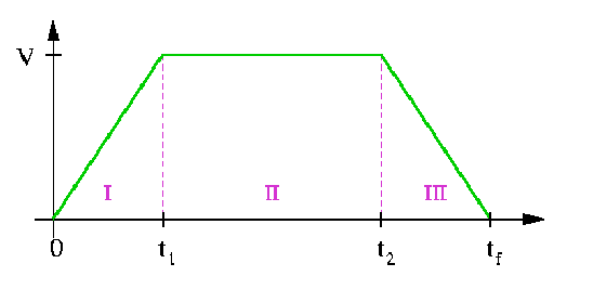
\includegraphics[scale=0.5]{vt.png}
	\captionof{figure}{\textit{La vitesse du robot $v$ en fonction du temps $t$.\\}}
	\label{fig2} 
	\end{center} 
	
	\paragraph{Le travail préalable :} A partir de la courbe $v(t)$ on peut facilement obtenir l'équation du mouvement $y(t)$ en faisant une intégrantion : $ y(t) = \int v(t)dt $:\\
	
	\begin{center}
		$ y(t) = \overset{t}{\underset{0}{\int}}v(t)dt = \overset{t}{\underset{0}{\int}}\frac{V}{t_1}tdt = \frac{V}{2t_1} t^2 $ \hspace{1 cm} si $t \in [0, t_1].$\\[0.25 cm]
		
		$ y(t) = \overset{t}{\underset{t_1}{\int}}v(t)dt + \frac{V}{2} t_1 = \overset{t}{\underset{t_1}{\int}}V dt + \frac{V}{2} t_1 = V (t-t_1) + \frac{V}{2} t_1$ \hspace{1 cm} si $t \in ]t_1, t_2].$\\[0.25 cm]
		
		$ y(t) = \overset{t}{\underset{t_2}{\int}}v(t)dt + \frac{V}{2} t_1 + V (t_2-t_1) = \overset{t}{\underset{t_1}{\int}} \frac{V}{(t_f-t_2)}t + V(1+\frac{t_2}{t_f-t_2}) dt + \frac{V}{2} t_1 + V (t_2-t_1) =$\\[0.25 cm] $ \frac{-V}{2t_1}t^2 + V (1+\frac{t_1}{t_2})t + [\frac{V}{2t_1}t^{2}_2 - V(1+\frac{t_2}{t_1})t_2 + \frac{V}{2} t_1 + V (t_2-t_1)]$ \hspace{1 cm} si $t \in ]t_2, t_f].$			
			 
	\end{center} 
	 \par Arrivés là il ne reste qu'à calculer $y*=y(t_f)$ et ainsi écrire la relation qui unit $V,\hspace{1 mm} t_f, \hspace{ 1 mm} t_1$ et $y*$:
	 
	 \begin{center}
	 	
		$y* = y(t_f) = \frac{-V}{2t_1}t^2_f + V (1+\frac{t_1}{t_2})t_f + [\frac{V}{2t_1}t^{2}_2 - V(1+\frac{t_2}{t_1})t_2 + \frac{V}{2} t_1 + V (t_2-t_1)]$	 	
	 \end{center} 
	 
	  \paragraph{} Comme on sait que: $t_2 = t_f-t_1$ alors: \\
	  
		 \begin{center}
			
				$y* = \frac{-V}{2t_1}t^2_f + V (1+\frac{t_1}{t_f-t_1})t_f + [\frac{V}{2t_1}(t_f-t_1)^2 - V(1+\frac{t_f-t_1}{t_1})(t_f-t_1) + \frac{V}{2} t_1 + V (t_f-2t_1)]$		
			 
		\end{center}		  
	  
\section{\textsc{Partie programme}} 

	\paragraph{} La commande utilisée sera par conséquent une commande en vitesse appliquée à l’ensemble des deux
moteurs de $Pekee$. Le programme demandera à l’utilisateur la vitesse $(en cm/s)$, la durée des périodes d’accélération/décélération $(en ms)$ et indiquera la distance que devrait parcourir le robot.\\
\textbf{Nota:} $V=1m/s = 0.1cm/ms$, l'utilisateur ne doit en aucun cas appliquer une vitesse au dessus de $V$.

\paragraph{Création de la classe MyLoopHandlerClass\\[0.25 cm]}

\begin{lstlisting}

MyLoopHandlerClass::MyLoopHandlerClass(int t0,int t1,int tf,float vmax):out("trajectoire.txt") // vitesse.txt pour le trace de la vitesse
{
	this -> T1=t1; //ms
	this -> Tf=tf; //ms
	this -> Vmax=vmax; // Vmax = 0.1 cm/ms
	this -> T0=t0;
	
}

MyLoopHandlerClass::~MyLoopHandlerClass(void)
{
}

bool MyLoopHandlerClass::OnLoop(void)
 {	
	int t = GetTickCount()-T0-20;//le -20ms nous rapproche plus du t=0s
	double D,V;//distance et Vitesse 
	
	if (t <= T1)
	{
		D =  0.5*Vmax*t*t/T1; // cm
		V= t*Vmax/T1;  
	}
	if((t>T1) && (t<=Tf-T1))
	{
		D=  0.5*Vmax*T1+Vmax*(t-T1); // cm
		V=Vmax;
	} 
	if(t>Tf-T1 && t<=Tf)
	{
	
		D =   0.5*Vmax*T1+Vmax*(Tf-T1-T1)+ 0.5*Vmax/T1*((Tf-T1)*(Tf-T1)-t*t) + Vmax*Tf/T1*(t-(Tf-T1));//cm 
		V=-Vmax+((Vmax/(Tf-T1-Tf))*(t-Tf-T1));
		
	}
	cout << t << " ms\t" << V << " cm/s\t"<< D <<"cm"<< std::endl; // affichage sur le terminal de la distance parcourue et de la vitesse instantanee chaque 20 ms.
	out << t << "\t" << D << "\t" <<V << std::endl;  
	
	/* ecriture sur le fichier trajectoire.txt, selectionner la colonne 1 et 2 pour tracer y(t) via Gnuplot ou au 			meme temps on selectionne la colonne 1 et 3 pour tracer v(t) */    

	return true;
}

 void MyLoopHandlerClass:: OnStopped ()
 {
	 out.close();
 }

\end{lstlisting}	

\paragraph{Les modifications apportées sur le main : maeva\text{\_}sql\\[0.25 cm]}

\begin{lstlisting}	

	  // --------------------------------- Initialisation du Timer
		int TT0=GetTickCount();
		MyLoopHandlerClass *handler = new MyLoopHandlerClass (TT0,TT1,TTf,VVmax);
		CMultimediaTimer timer(*handler);

		timer.Start(20,1);

	  // --------------------------------- Tracage de la Position

		while (!kbhit()) {Sleep(1); Pekee.SetSpeed(100,0) ;}
 
	  // --------------------------------- Arret du Timer
		
		timer.Stop();

	  // Arret de la connexion au Robot

		Pekee.Disconnect();
	
\end{lstlisting}	

\par Avec le fichier trajectoire.txt et le fichier vitesse.txt remplis, on pourra maitenant tracer ces deux courbes via Gnuplot. Pour $t_1=1000ms, \hspace{1 mm} t_f= 3000ms \hspace{1 mm} et \hspace{1 mm} V= 0.1cm/ms=1m/s$ on trouve :\\
   
   	\begin{center}
	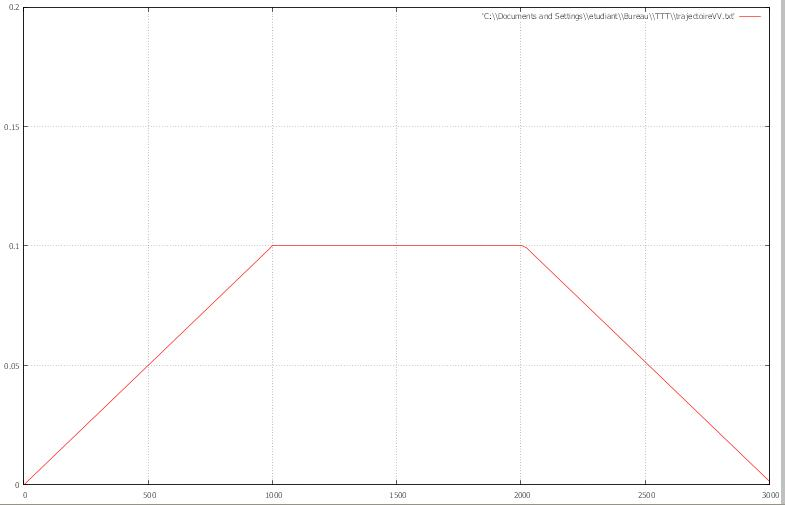
\includegraphics[scale=0.6]{V.JPG}
	\captionof{figure}{\textit{La vitesse du robot $v$ en fonction du temps $t$ via Gnuplot.\\}}
	\label{fig3} 
	\end{center}
	 
	\par La courbe de la vitesse correspond parfaitement à celle du cahier des charges. 

	 \begin{center}
	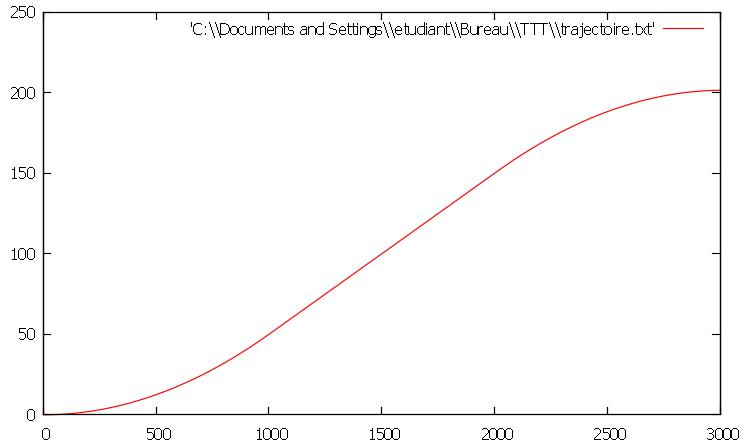
\includegraphics[scale=0.6]{Y.JPG}
	\captionof{figure}{\textit{La trajectoire du robot $v$ en fonction du temps $t$ via Gnuplot.\\}}
	\label{fig4} 
	\end{center}
	
	\textbf{Nota:} On vous invite à zoomer vers les 200 \text{\%} sur les figures précédentes pour plus de clarté.\\
	
	\textbf{Nota:} Les fichiers : MyloopHandlerClass.h, MyloopHandlerClass.cpp en entier et maeva\text{\_}sql.cpp en entier sont à trouver dans les annexes.\\ 		
	
	\chapter*{\textsc{Conclusion}}
	\addcontentsline{toc}{chapter}{\textsc{Conclusion}}

	\paragraph{} A défaut de temps nous n'avons pas pu réussir et faire toutes les demandes du cahier des charges néaumoins nous avons acquis le savoir de simuler et de commander un robot à base du C++ et ainsi approfondir nos connaissances sur ce dernier.